\subsection{}
This Exercise has been implemented in "Q0013.py".
\subsection{}
I have been unable to get the code for the "Divided Differences" and "Newton-Horner" algorithms to work in the Q files, as the book pseudocode is not very clear. The plot for the Newton-Horner algorithm is then for one that does almost the right thing, except all the values are significantly further from zero than they should be. The general form of the function is correct though, and it has a running time extremely close to what the correct one would have.\\
However, I can still comment on what I think would happen, if they were implemented. Based purely on the number of iterations the algorithms go through, it would seem like the Lagrange polynomial function would be slowest, as it will loop through $(n * (n-1))$ elements in total, whereas the other two reduce the second factor significantly by limiting the second loop to $n-j$ iterations instead of $n-1$. This means that while all the algorithms have an $O(n^2)$ asymptotic running time, the Lagrangian one has significantly larger constant factors. In the plot below, we can see that the running time is polynomial for both algorithms, as expected, and that the Newton-Horner method is significantly faster, but only with regards to constant factors. Any significant outliers are likely due to cache misses inside the computer.\\
\begin{figure}[ht]
  \caption{Lagrangian method}
  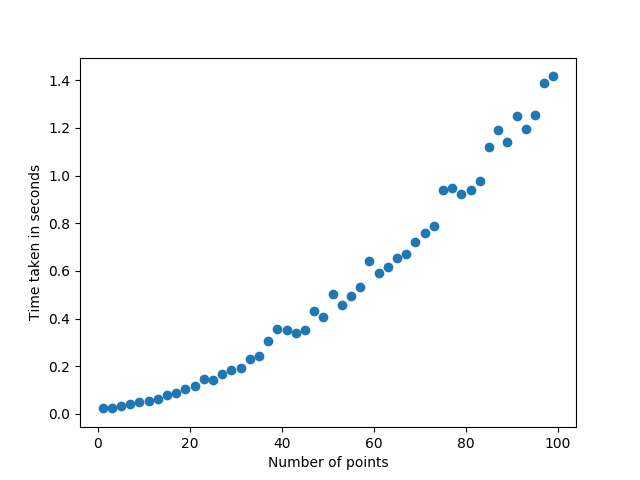
\includegraphics[width=\linewidth]{timeplot}
\end{figure}
\begin{figure}[ht]
  \caption{Incorrect Newton-Horner method}
  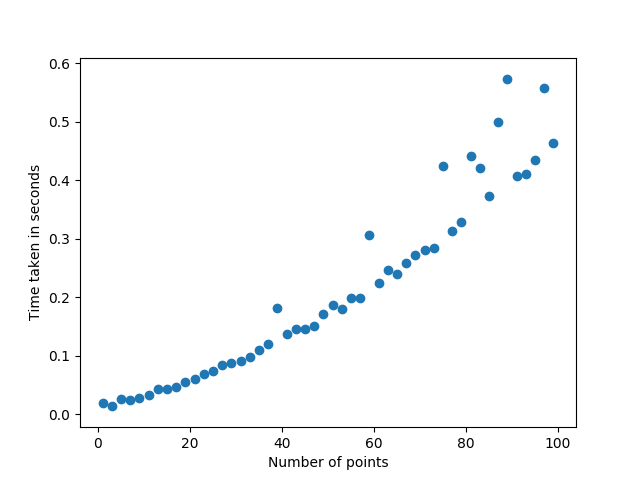
\includegraphics[width=\linewidth]{timeplot_newton}
\end{figure}
